%
% ---------------------------------------------------------------
% Copyright (C) 2012-2018 Gang Li
% ---------------------------------------------------------------
%
% This work is the default powerdot-tuliplab style test file and may be
% distributed and/or modified under the conditions of the LaTeX Project Public
% License, either version 1.3 of this license or (at your option) any later
% version. The latest version of this license is in
% http://www.latex-project.org/lppl.txt and version 1.3 or later is part of all
% distributions of LaTeX version 2003/12/01 or later.
%
% This work has the LPPL maintenance status "maintained".
%
% This Current Maintainer of this work is Gang Li.
%
%

\documentclass[
 size=12pt,
 paper=smartboard,  %a4paper, smartboard, screen
 mode=present, 		%present, handout, print
 display=slides, 	% slidesnotes, notes, slides
 style=tuliplab,  	% TULIP Lab style
 pauseslide,
 fleqn,leqno]{powerdot}


\usepackage{cancel}
\usepackage{caption}
\usepackage{stackengine}
\usepackage{smartdiagram}
\usepackage{attrib}
\usepackage{amssymb}
\usepackage{amsmath} 
\usepackage{amsthm} 
\usepackage{mathtools}
\usepackage{rotating}
\usepackage{graphicx}
\usepackage{boxedminipage}
\usepackage{rotate}
\usepackage{calc}
\usepackage[absolute]{textpos}
\usepackage{psfrag,overpic}
\usepackage{fouriernc}
\usepackage{pstricks,pst-3d,pst-grad,pstricks-add,pst-text,pst-node,pst-tree}
\usepackage{moreverb,epsfig,subfigure}
\usepackage{color}
\usepackage{booktabs}
\usepackage{etex}
\usepackage{breqn}
\usepackage{multirow}
\usepackage{natbib}
\usepackage{bibentry}
\usepackage{gitinfo2}
\usepackage{siunitx}
\usepackage{nicefrac}
%\usepackage{geometry}
%\geometry{verbose,letterpaper}
\usepackage{media9}
\usepackage{animate}
%\usepackage{movie15}
\usepackage{auto-pst-pdf}

\usepackage{breakurl}
\usepackage{fontawesome}
\usepackage{xcolor}
\usepackage{multicol}



\usepackage{verbatim}
\usepackage[utf8]{inputenc}
\usepackage{dtk-logos}
\usepackage{tikz}
\usepackage{adigraph}
%\usepackage{tkz-graph}
\usepackage{hyperref}
%\usepackage{ulem}
\usepackage{pgfplots}
\usepackage{verbatim}
\usepackage{fontawesome}


\usepackage{todonotes}
% \usepackage{pst-rel-points}
\usepackage{animate}
\usepackage{fontawesome}

\usepackage{listings}
\lstset{frameround=fttt,
frame=trBL,
stringstyle=\ttfamily,
backgroundcolor=\color{yellow!20},
basicstyle=\footnotesize\ttfamily}
\lstnewenvironment{code}{
\lstset{frame=single,escapeinside=`',
backgroundcolor=\color{yellow!20},
basicstyle=\footnotesize\ttfamily}
}{}


\usepackage{hyperref}
\hypersetup{ % TODO: PDF meta Data
  pdftitle={Presentation Title},
  pdfauthor={Gang Li},
  pdfpagemode={FullScreen},
  pdfborder={0 0 0}
}
\usepackage{setspace} 

% \usepackage{auto-pst-pdf}
% package to show source code

\definecolor{LightGray}{rgb}{0.9,0.9,0.9}
\newlength{\pixel}\setlength\pixel{0.000714285714\slidewidth}
\setlength{\TPHorizModule}{\slidewidth}
\setlength{\TPVertModule}{\slideheight}
\newcommand\highlight[1]{\fbox{#1}}
\newcommand\icite[1]{{\footnotesize [#1]}}

\newcommand\twotonebox[2]{\fcolorbox{pdcolor2}{pdcolor2}
{#1\vphantom{#2}}\fcolorbox{pdcolor2}{white}{#2\vphantom{#1}}}
\newcommand\twotoneboxo[2]{\fcolorbox{pdcolor2}{pdcolor2}
{#1}\fcolorbox{pdcolor2}{white}{#2}}
\newcommand\vpspace[1]{\vphantom{\vspace{#1}}}
\newcommand\hpspace[1]{\hphantom{\hspace{#1}}}
\newcommand\COMMENT[1]{}

\newcommand\placepos[3]{\hbox to\z@{\kern#1
        \raisebox{-#2}[\z@][\z@]{#3}\hss}\ignorespaces}

% \renewcommand{\baselinestretch}{1.2}
\renewcommand{\baselinestretch}{1.2}

\newcommand{\draftnote}[3]{
	\todo[author=#2,color=#1!30,size=\footnotesize]{\textsf{#3}}	}
% TODO: add yourself here:
%
\newcommand{\gangli}[1]{\draftnote{blue}{GLi:}{#1}}
\newcommand{\shaoni}[1]{\draftnote{green}{sn:}{#1}}
\newcommand{\gliMarker}
	{\todo[author=GLi,size=\tiny,inline,color=blue!40]
	{Gang Li has worked up to here.}}
\newcommand{\snMarker}
	{\todo[author=Sn,size=\tiny,inline,color=green!40]
	{Shaoni has worked up to here.}}

%%%%%%%%%%%%%%%%%%%%%%%%%%%%%%%%%%%%%%%%%%%%%%%%%%%%%%%%%%%%%%%%%%%%%%%%
% title
% TODO: Customize to your Own Title, Name, Address
%
\title{Flip00 Presentation}
\author{
Huanhuan Ge
\\
\\Qingdao University of Technology
}
\date{\gitCommitterDate}


% Customize the setting of slides
\pdsetup{
% TODO: Customize the left footer, and right footer
rf=\href{http://www.tulip.org.au}{
Last Changed by: \textsc{\gitCommitterDate}
},
cf={Flip00 Presentation},
}


\begin{document}

\maketitle

%\begin{slide}{Overview}
%\tableofcontents[content=sections]
%\end{slide}


%%==========================================================================================
%%
\begin{slide}[toc=,bm=]{Overview}
\begin{spacing}{1.00}
\tableofcontents[content=currentsection,type=1]
\end{spacing}
\end{slide}
%%
%%==========================================================================================


\section{Problem}


%%==========================================================================================
%%
\begin{slide}{Description and Evaluation}
% \begin{center}
% \twotonebox{\rotatebox{90}{Description}}{\parbox{.86\textwidth}
% {Predict Future Sales by giving a time-series dataset consisting of daily sales data.
% }}
% % \twotonebox{\rotatebox{90}{Evaluation}}{\parbox{.86\textwidth}
% % {Root mean squared error (RMSE). \\
% %  True target values are clipped into [0,20] range.
% % }}
% \end{center}
\begin{center}
  \twotonebox{\rotatebox{0}{Description}}{\parbox{.80\textwidth}
  {Predict Future Sales by giving a time-series dataset consisting of daily sales data.
  }}
\bigskip
  \twotonebox{\rotatebox{0}{Evaluation}}{\parbox{.80\textwidth}
  {Root mean squared error (RMSE). \\
  True target values are clipped into [0,20] range.
  }}
\end{center}

% \bigskip
% \begin{center}
% \begin{tabular}{c| c c c c }
% \toprule
% Player & \texttt{3PT\%}  & \texttt{FTA} & \texttt{FT\%} & \texttt{To} \\
% \midrule
% $P_1$
% &  {$65$} &  {$4$} &  {$33$} &  {$8$} \\
% $P_2$
% &  {$78$} &  {$1$}&  {$65$}&  {$5$} \\
% $P_3$
% &  {$58$} &  {$6$} &  {$46$} &  {$3$} \\
% $P_4$
% &  {$68$} &  {$1.2$}&  {$85$}&  {$6.2$} \\
% $P_5$
% &  {$58$} &  {$6.2$} &  {$36$} &  {$3.4$}\\
% \bottomrule
% \end{tabular}
% \end{center}
% \bigskip

%%==========================================================================================
\begin{note}
First, I will introduce the problem definition.
In the real life,
a teacher may be interested in the characteristics that
make one student obvious different from others.
Or,
NBA sports coaches would prefer to
know the advantages and disadvantages of one player.
Here, the player can be regarded as a query object.

For example, team A has five players,
each player has four features.
The NBA sports coaches may want to know the features of
player $1$ that are different from others.

The above example can be seen as outlying aspects mining.
The main purpose of outlying aspects mining is to identify
the outstanding features of the query object.
\end{note}
%%==========================================================================================

\end{slide}
%%
%%==========================================================================================


%%==========================================================================================
%%
\section{Data Processing}

\begin{slide}{Basic Information of Data}
\begin{center}
\setlength{\belowdisplayskip}{0pt}
\setlength{\abovedisplayskip}{0pt}
% \begin{tabular}{p{5cm}p{8cm}p{6cm}}
\begin{table}[h!]
\setlength{\belowdisplayskip}{0pt}
\setlength{\abovedisplayskip}{0pt}
\setlength{\abovecaptionskip}{0pt}
\setlength{\belowcaptionskip}{0pt}
\centering
\small
\caption{Data}
\resizebox{.92\textwidth}{25mm}{
\begin{tabular}{p{5cm}p{8cm}p{8cm}}
\toprule
\centering
Name
& Description & Attribute \\
\midrule

\centering 
sales_train.csv
& { Training set(data from January 2013 to October 2015)} &  {date,date_block_num,shop_id,item_id, item_price,item_cnt_day}  \\
\centering 
test.csv
& {Test set(Predict sale in November2015)} &  {ID,shop_id,item_id} \\
\centering 
items.csv
&  {Supplementary information of products} &  {item_name,item_id,item_category_id}   \\
\centering 
shops.csv
&  {Supplementary information of shops} &  {shops_name,shops_id} \\
\centering 
item_categories.csv
&  {Supplementary information of item categories} &  {item_categories_name,item_categories_id} \\
\centering
sample_submission.csv
&  {Format of submission} &  {ID,item_cnt_month} \\
\bottomrule
\end{tabular}}
\end{table}
\end{center}
\vspace{.1mm}
\twocolumn{
  \begin{itemize}
    \item
    % Explain the distinctive \textcolor{orange}{aspects} of the query object.
    There are 2935849 lines in train set. \\
    \smallskip
    There are 214200 lines in test set.\\
    \end{itemize}}
    {
      \begin{itemize}
        \item
        % Find out \textcolor{orange}{all} unusual
        % \textcolor{orange}{objects} in the whole dataset.
        There are 21807 unique items in train set.\\
        \smallskip
        % \textcolor{orange}{No} explanation on how they are different.
        There are 60 unique shops in train set.\\
        \smallskip
        There are 5100 unique items in test set.\\
        \smallskip
        There are 42 unique shops in test set.\\
        \smallskip
        \end{itemize}
    }
 




%%==========================================================================================
\begin{note}
Based on the above example,
I will compare the differences
between outlying aspects mining and outlier detection.

Outlying aspects mining aims to
explain the distinctive aspects of the query object.
The query object may or may not be an outlier.
In contrast,
Outlier detection aims to discover all possible
outlying objects in the dataset.
Without explaining how and why they are different.

Let's go back to the NBA example,
in that example,
the output of the outlying aspects mining may be
a combination of four features,
but the output of the outlier detection may be any of those five players.
\end{note}
%%==========================================================================================

\end{slide}
%%
%%==========================================================================================


%%==========================================================================================
%%
\begin{slide}{Missing Value and NaN Value}
  \onecolumn{
    \begin{figure}
      \centering
      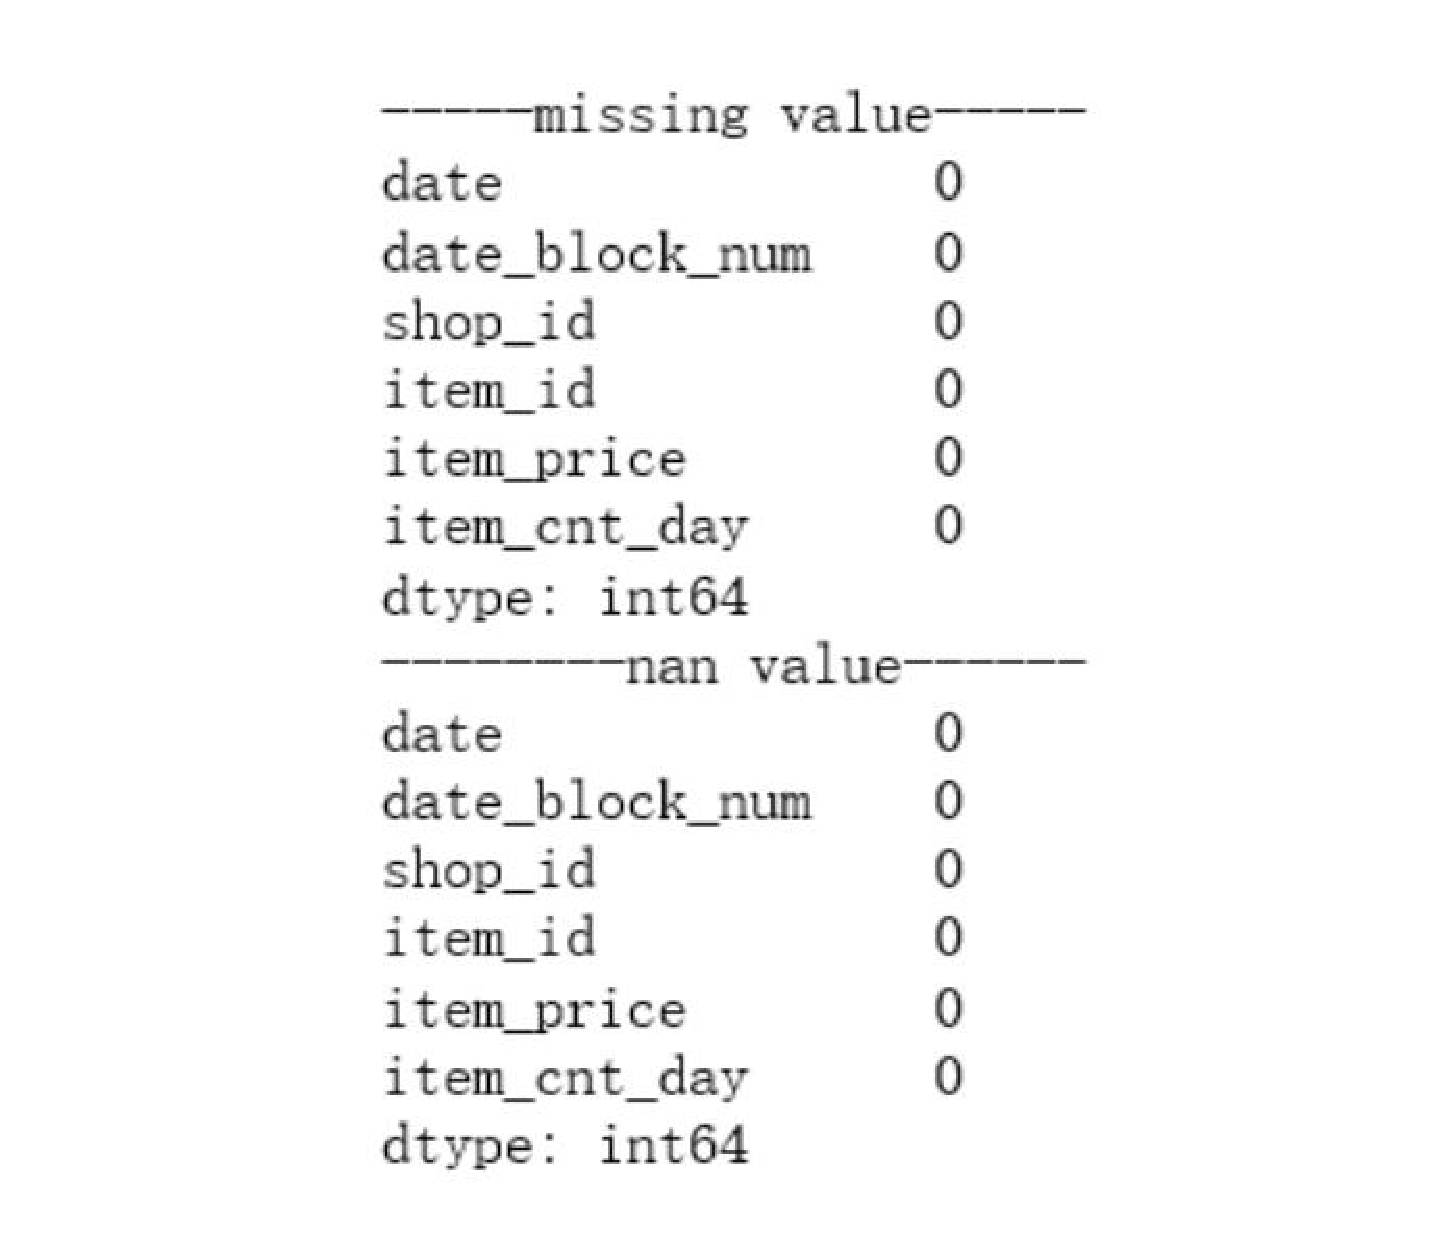
\includegraphics[width=0.6\textwidth]{figures/Figure1.eps}\\
      \caption{Missing Value and NaN Value}
    \end{figure}
    }
% \twocolumn{
% \begin{figure}
%   \centering
%   \selectcolormodel{rgb}
%   \missingfigure{Testing.}
%   %\includegraphics[width=0.6\textwidth]{figures//demical.eps}\\
%   \caption{Medical}\label{fig:demical}
% \end{figure}
% }{
% \begin{figure}
%   \centering
%   \selectcolormodel{rgb}
%   \missingfigure{Testing.}
%   %\includegraphics[width=0.6\textwidth]{figures//NBA_team.eps}\\
%   \caption{NBA-Team}\label{fig:timg}
% \end{figure}
% }

%%==========================================================================================
\begin{note}
However,
there is such a phenomenon in real life.
Doctors desire to identify the characteristics between
a group of cancer patients and normal people.
NBA coaches are passionate about exploring the obvious strengths and
weaknesses of the team compared with other teams.

Based on such a phenomenon in the real life,
we proposed the concept of group outlying aspects mining.
\end{note}
%%==========================================================================================

\end{slide}
%%
%%==========================================================================================


%%==========================================================================================
%%
\begin{slide}{Outliers and Duplicate Data}
% \begin{slide}[toc=,bm=]{Outliers and Duplicate Data}
\begin{itemize}
  \item
  There are 2935849 lines in train set. \\
  \smallskip
  There are 214200 lines in test set.\\
\end{itemize}
\vspace{0.75cm}
  \begin{figure}[htbp]
    \centering
    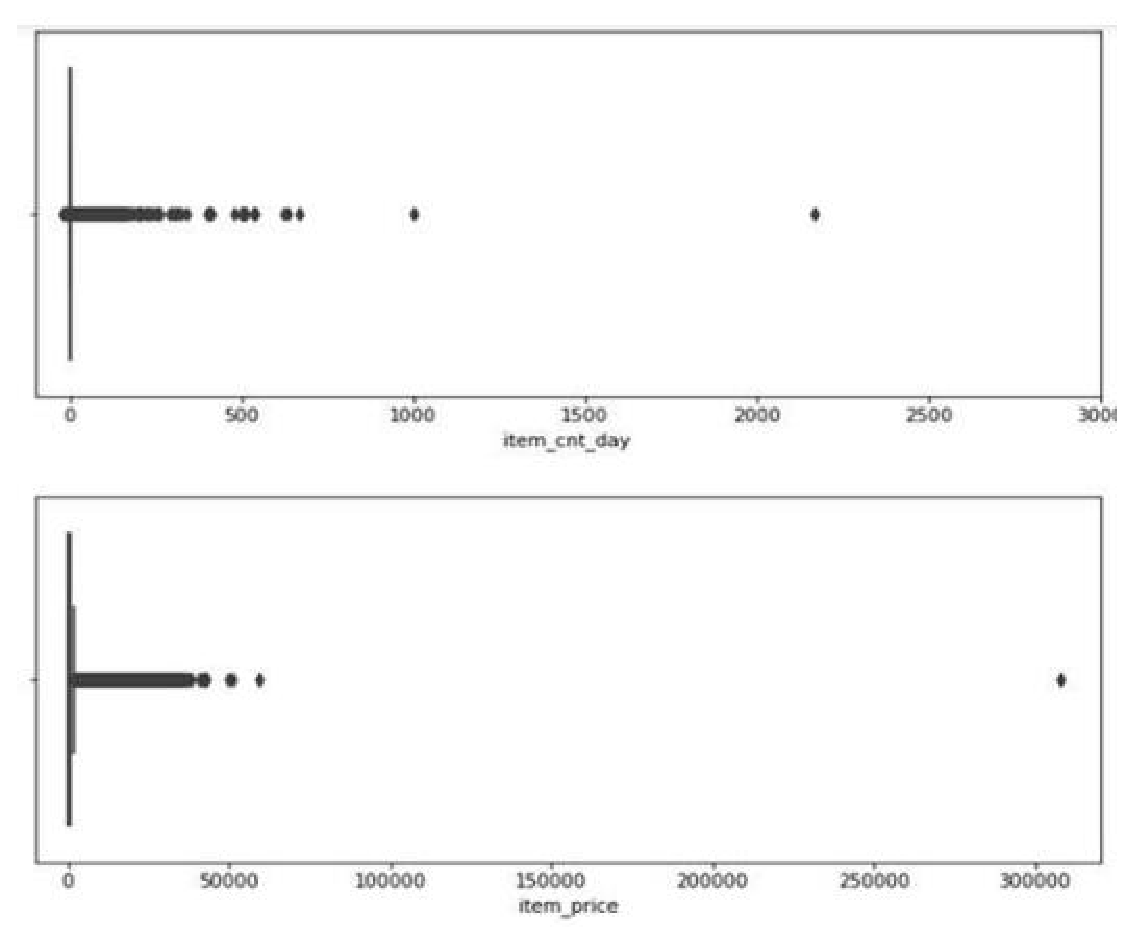
\includegraphics[width=0.5\textwidth,height=0.4\textwidth]{figures/Figure2.eps}\\
    \caption{Outliers Data}
  \end{figure}
    
 

%%==========================================================================================
\begin{note}
Next,
let me talk about the concept of group outlying aspects mining.

For example,
Dataset $G$ has $n$ groups.
$G_q$ is the query group.
and other groups are comparison groups.
Each object in the group has d features $F = $ $f_1$, $f_2$, $f_3$ to $f_d$.
The group outlying aspects mining is to identify the top-k group outlying subspaces,
which are different from other groups.

What does the top-k group outlying subspaces mean?
Next, I will explain it.
\end{note}

%%==========================================================================================
\end{slide}
%%
%%==========================================================================================


%%==========================================================================================
%%
\begin{slide}{Process Shops Set}

\begin{itemize}
\item
Same shop name, different shop ID \\
39 and 40,10 and 11,0 and 57, 58 and 1
\item
Modify the ID based on the test
\item
Shop full name: shop’s city-shop’s type-shop’s name
\item
Encode shops information
\end{itemize}

\vspace{0.75cm}
\begin{figure}[htbp]
  \centering
  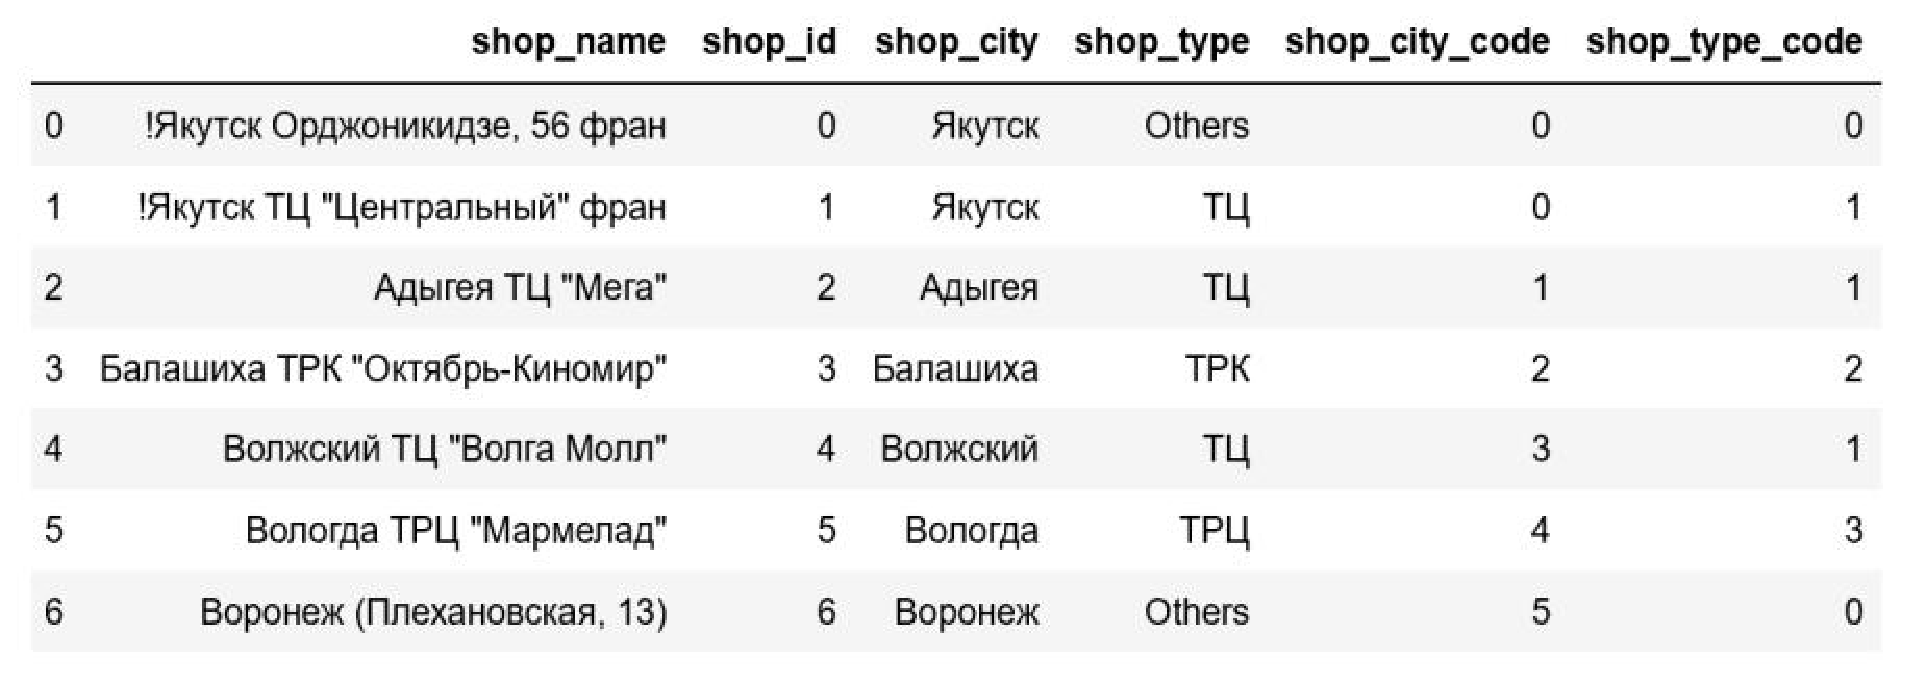
\includegraphics[width=0.8\textwidth,height=0.3\textwidth]{figures/Figure3.eps}\\
  \caption{Encode Shops Information}
\end{figure}

% \begin{figure}[htbp]
%     \centering
%     \subfigure[Original Feature Spaces]{
%       \selectcolormodel{rgb}
%       \missingfigure[figwidth=5.5cm]{Test.}
%         %\includegraphics[width=0.3\textwidth]{figures//example-basketball-original.eps}
%         \label{fig:basketball-original}
%     }
%     \subfigure[Group Outlying Spaces]{
%        \selectcolormodel{rgb}
%        \missingfigure[figwidth=5.5cm]{Test.}
%         %\includegraphics[width=0.3\textwidth]{figures//example-basketball-projection.eps}
%         \label{fig:basketball-projection}
%     }
%     \subfigure[Another Subspaces]{
%       \selectcolormodel{rgb}
%       \missingfigure[figwidth=5.5cm]{Test.}
%         %\includegraphics[width=0.28\textwidth]{figures//basketball-another-subspaces.eps}
%         \label{fig:basketball-projection1}
%     }
% %    \caption{Histogram representation of a group on three single features}
%     \label{fig:Basketball-Example}
% \end{figure}

%%==========================================================================================
\begin{note}
We use $\rho_s(\cdot)$ to describe an outlying scoring function.
$\rho_s(\cdot)$ quantifies the outlying degree of the query group in a subspaces $s$.
In addition,
we use the scoring function to make a descending order and at last
filter out the top k group outlying subspaces.
It is obvious that the outlying subspaces make the
query group different from other groups.
\end{note}
%%==========================================================================================

\end{slide}
%%
%%==========================================================================================


%%==========================================================================================
%%
\begin{slide}{Process Items Set}
\begin{itemize}
\item
\smallskip
Same item name, different item ID \\
2514 and 2558,2968 and 2970,5061 and 5063, 14537 and 14539,19465 and 19475,19579 and 19581
\item
Modify the ID based on the test
\end{itemize}



%%==========================================================================================
\begin{note}
In order to identify the top-k outlying subspaces,
we categorize the features into $2$ non-overlapping groups,
trivial outlying features and non-trivial outlying subspaces.

First, let me introduce the trivial outlying features.

Trivial outlying features are one-dimension subspaces.
In the subspace,
the query group's outlying degree is larger than the threshold $\alpha$.

We can see from table $1$,
when the specified threshold $\alpha = 4$,
the trivial outlying feature is \{$F_1$\}.
\end{note}
%%==========================================================================================

\end{slide}
%%
%%==========================================================================================


%%==========================================================================================
%%
\begin{slide}{Process Categories Set}
\begin{itemize}
\item
\smallskip
Shop full name: category’s type-category’s subtype.
\item
\smallskip
Encode categories information
\end{itemize}

\vspace{0.75cm}
\begin{figure}[htbp]
  \centering
  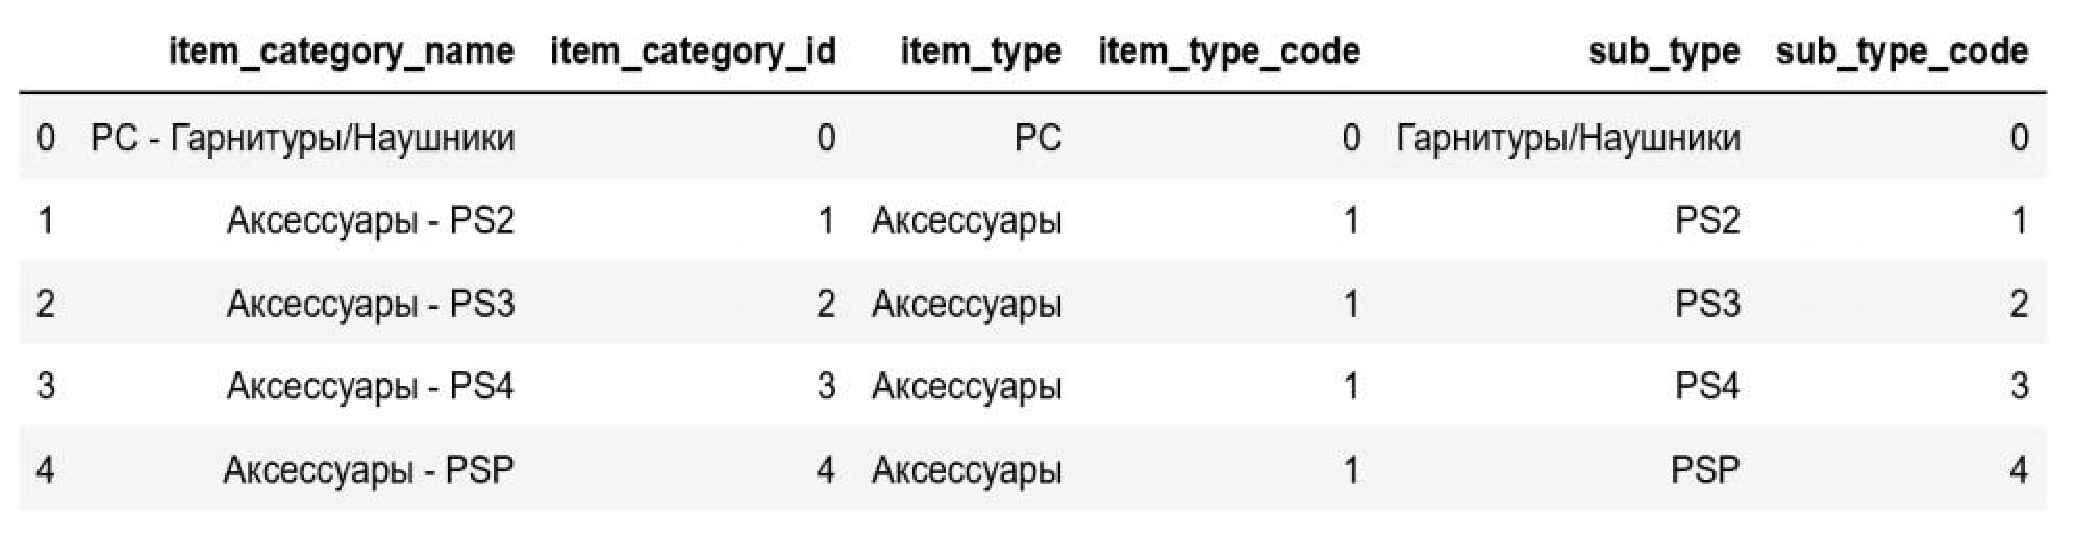
\includegraphics[width=0.8\textwidth,height=0.3\textwidth]{figures/Figure4.eps}\\
  \caption{Encode Categories Information}
\end{figure}

% \begin{table}
% \setlength{\abovecaptionskip}{0pt}
% \setlength{\belowcaptionskip}{10pt}
% \centering
% \caption{$\alpha = 4$}

% \begin{tabular}{  c  |  c }
% \toprule
% \centering
% \texttt{Feature}  & \texttt{Outlying Degree}  \\
% \midrule
%  {\{$F_1$\}}                           & $4.351$ \\
%  {\textcolor{orange}{\{$F_3, F_4$\}}}  & $4.024$ \\
%  {\{$F_2, F_4$\}}                      & $2.318$ \\
%  {\{$F_2$\}}                           & $2.002$ \\
%  {\{$F_3$\}}                           & $1.028$ \\
% \bottomrule
% \end{tabular}
% \end{table}

%%==========================================================================================
\begin{note}
Next,
I will introduce the non-trivial outlying subspaces.
Non-Trivial outlying subspaces are multi-dimension subspaces.
In the subspace,
the query group's outlying degree is larger than the threshold $\alpha$.

Table $2$ shows that,
when the threshold $\alpha$ equal four,
the non-trivial outlying subspace is \{$F_3$, $F_4$\}.
\end{note}
%%==========================================================================================

\end{slide}
%%
%%==========================================================================================
%%
\begin{slide}{Sales Analysis}
  \begin{figure}[htbp]
    \centering
    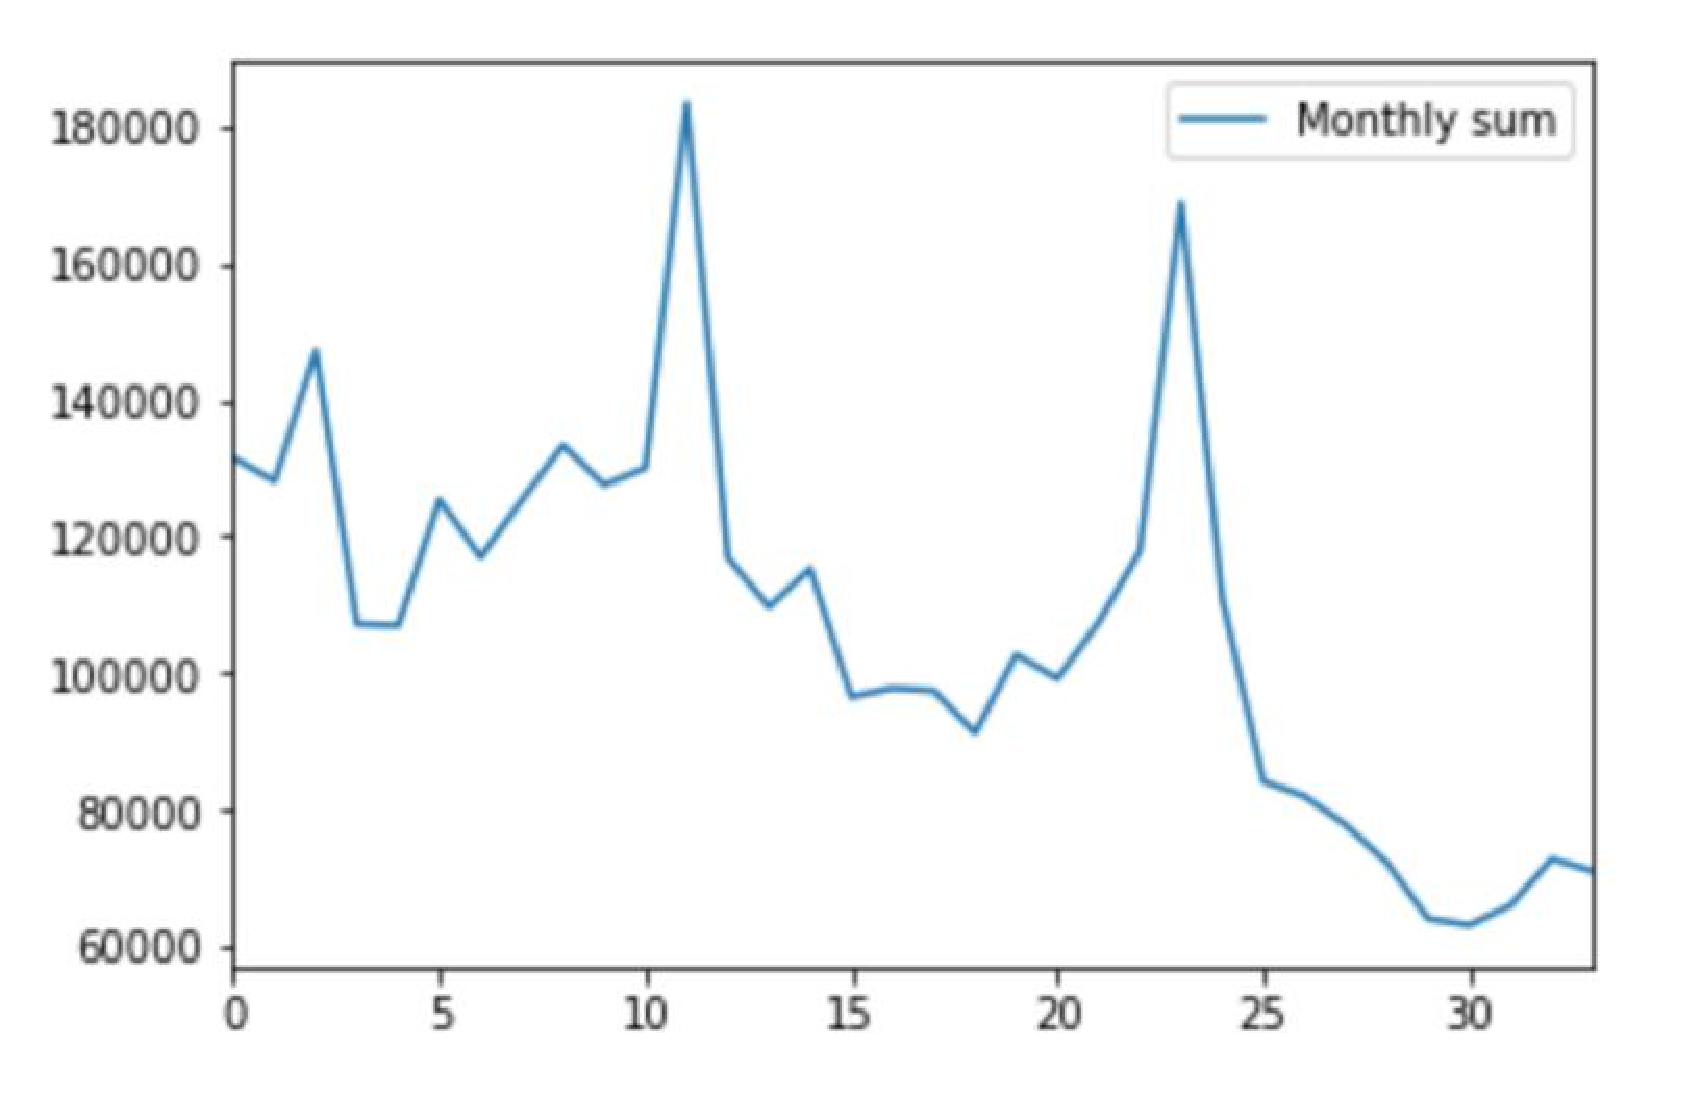
\includegraphics[width=0.8\textwidth,height=0.5\textwidth]{figures/Figure5.eps}\\
    \caption{Total Sales Over Time}
  \end{figure}
  
  %%==========================================================================================
  \begin{note}
  Next,
  I will introduce the non-trivial outlying subspaces.
  Non-Trivial outlying subspaces are multi-dimension subspaces.
  In the subspace,
  the query group's outlying degree is larger than the threshold $\alpha$.
  
  Table $2$ shows that,
  when the threshold $\alpha$ equal four,
  the non-trivial outlying subspace is \{$F_3$, $F_4$\}.
  \end{note}
  %%==========================================================================================
  
  \end{slide}
  %%
  %%==========================================================================================
%%
\begin{slide}{Closed Shops and Discontinued Products}
\begin{itemize}
  \item
  \smallskip
  new shops:9,20,36 
  \item
  closed shops:0,1,8,11,13,17,23,27,29,30,32,33,40,43,51,54
\end{itemize}
\vspace{0.75cm}
\begin{figure}[htbp]
  \centering
  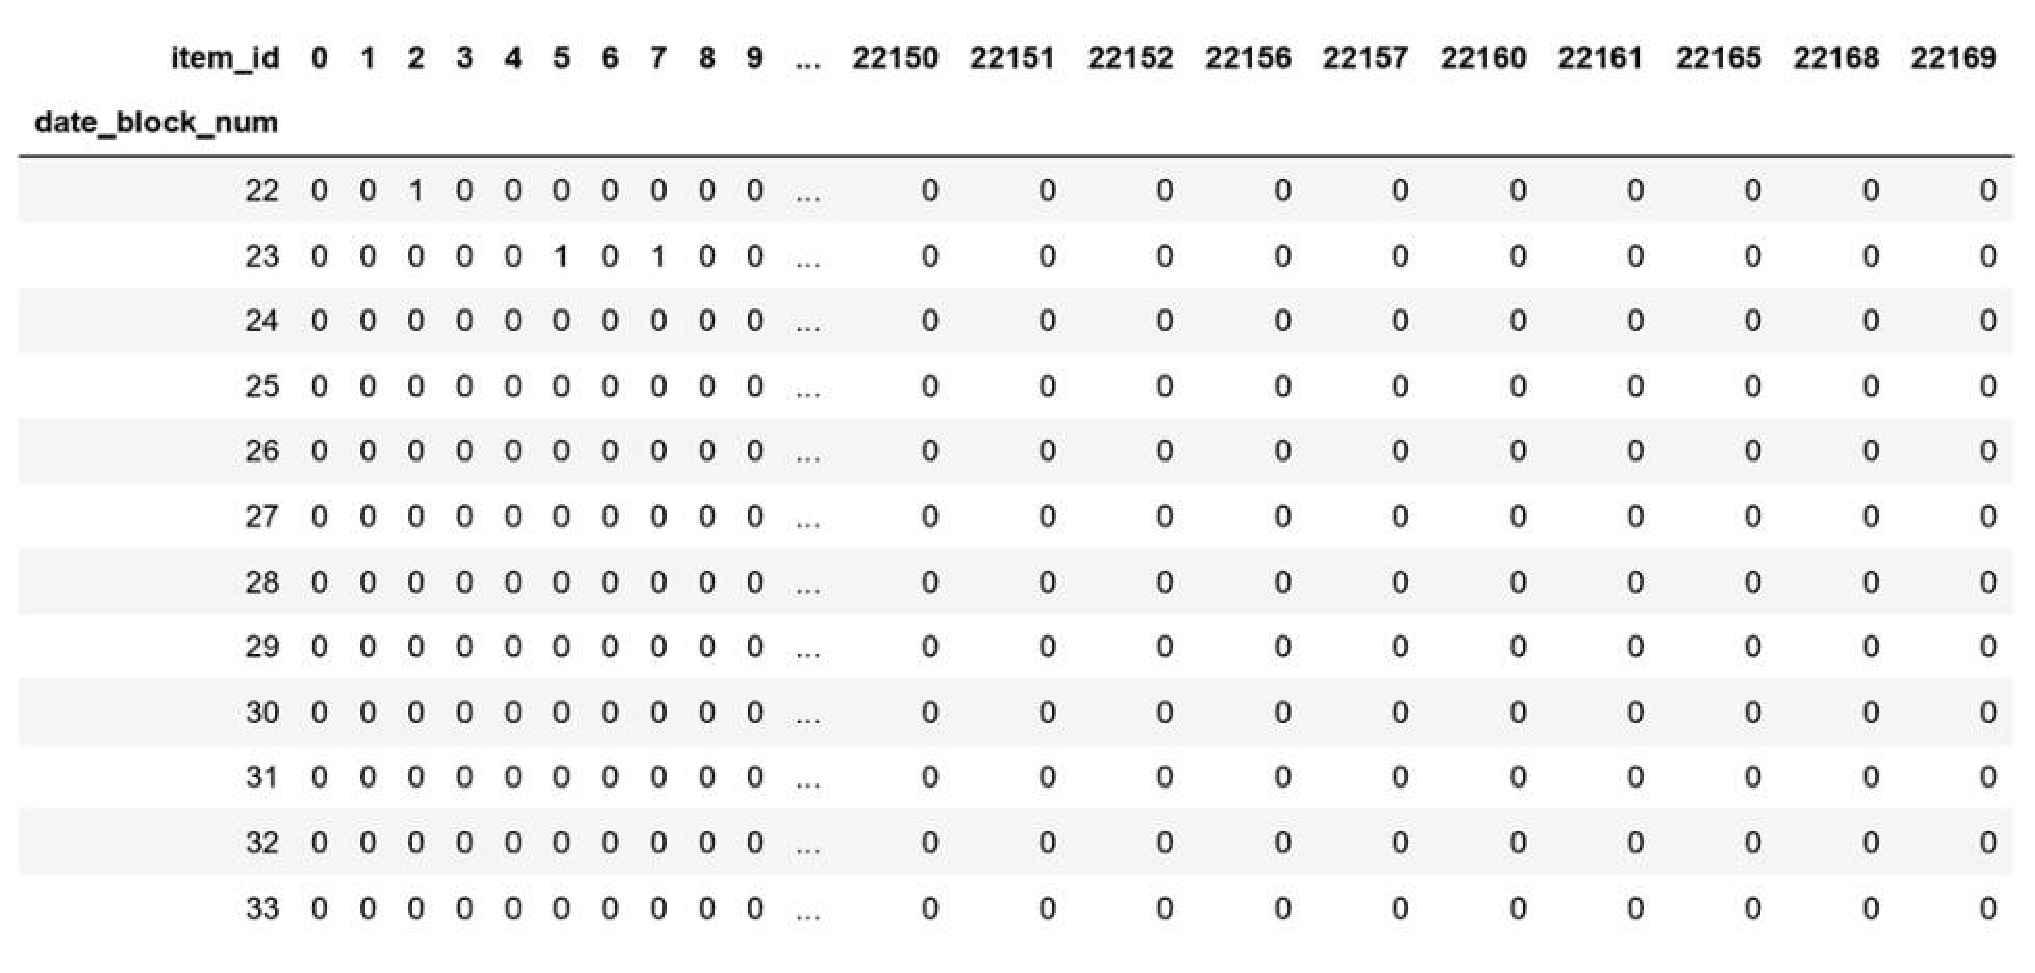
\includegraphics[width=0.8\textwidth,height=0.4\textwidth]{figures/Figure6.eps}\\
  \caption{Discontinued Products}
\end{figure}
  
  %%==========================================================================================
  \begin{note}
  In order to identify the top-k outlying subspaces,
  we categorize the features into $2$ non-overlapping groups,
  trivial outlying features and non-trivial outlying subspaces.
  
  First, let me introduce the trivial outlying features.
  
  Trivial outlying features are one-dimension subspaces.
  In the subspace,
  the query group's outlying degree is larger than the threshold $\alpha$.
  
  We can see from table $1$,
  when the specified threshold $\alpha = 4$,
  the trivial outlying feature is \{$F_1$\}.
  \end{note}
  %%==========================================================================================
  
  \end{slide}
  %%
  %%==========================================================================================
  
  
  %%==========================================================================================
  %%

\section{Feature Selection}
%%
\begin{slide}{Data Feature}
  \begin{itemize}
    \item
    \smallskip
    new shops:9,20,36 
    \item
    closed shops:0,1,8,11,13,17,23,27,29,30,32,33,40,43,51,54
  \end{itemize}
  \vspace{0.75cm}
  \begin{figure}[htbp]
    \centering
    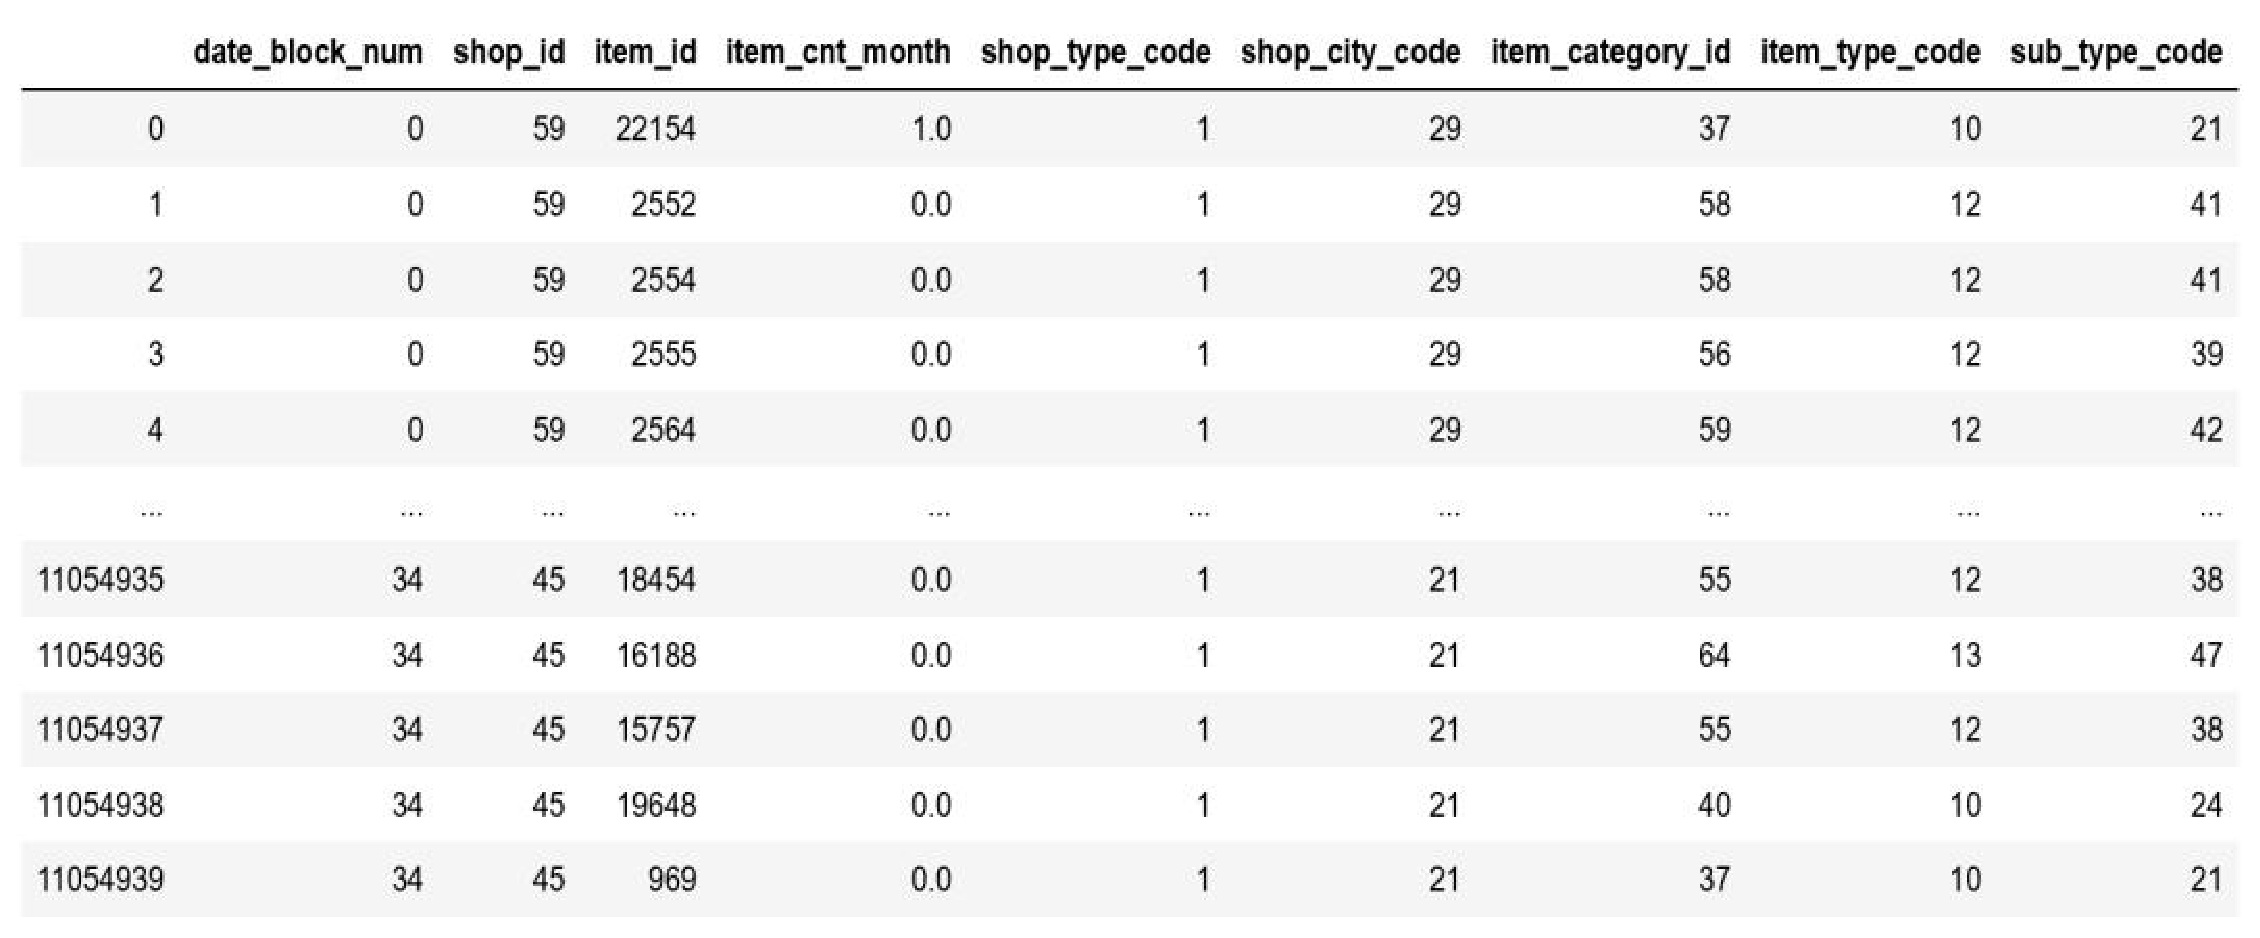
\includegraphics[width=0.8\textwidth,height=0.4\textwidth]{figures/Figure7.eps}\\
    \caption{Data Feature}
  \end{figure}
    
    %%==========================================================================================
    \begin{note}
    In order to identify the top-k outlying subspaces,
    we categorize the features into $2$ non-overlapping groups,
    trivial outlying features and non-trivial outlying subspaces.
    
    First, let me introduce the trivial outlying features.
    
    Trivial outlying features are one-dimension subspaces.
    In the subspace,
    the query group's outlying degree is larger than the threshold $\alpha$.
    
    We can see from table $1$,
    when the specified threshold $\alpha = 4$,
    the trivial outlying feature is \{$F_1$\}.
    \end{note}
    %%==========================================================================================
    
    \end{slide}
    %%

%%==========================================================================================
%%
\begin{slide}{Monthly Sales Feature}
  \begin{itemize}
    \item
    \smallskip
    average monthly sales of items
    \item
    average monthly sales of shops
    \item
    \smallskip
    average monthly sales of categories
    \item
    average monthly sales of types and subtypes
    \item
    \smallskip
    average monthly sales of shop’s city-item
    \item
    average monthly sales of shop’s type-item
  \end{itemize}
    
    %%==========================================================================================
    \begin{note}
    In order to identify the top-k outlying subspaces,
    we categorize the features into $2$ non-overlapping groups,
    trivial outlying features and non-trivial outlying subspaces.
    
    First, let me introduce the trivial outlying features.
    
    Trivial outlying features are one-dimension subspaces.
    In the subspace,
    the query group's outlying degree is larger than the threshold $\alpha$.
    
    We can see from table $1$,
    when the specified threshold $\alpha = 4$,
    the trivial outlying feature is \{$F_1$\}.
    \end{note}
    %%==========================================================================================
    
    \end{slide}
    %%

%%==========================================================================================
%%
\begin{slide}{Historical Feature}
  \begin{itemize}
    \item
    \smallskip
    Historical delay:1,2,3,6,12
    \item
    Historical Feature:
    \smallskip
  monthly sales of items \\
  average monthly sales of shops \\
  average monthly sales of items  \\
  average monthly sales of categories  \\
  average monthly sales of types and subtypes  \\
  average monthly sales of shop’s city-item   \\
  average monthly sales of shop’s type-item   \\
  \smallskip
    \item
    Delete the records in first 12 months and NAN records
  \end{itemize}
    
    %%==========================================================================================
    \begin{note}
    In order to identify the top-k outlying subspaces,
    we categorize the features into $2$ non-overlapping groups,
    trivial outlying features and non-trivial outlying subspaces.
    
    First, let me introduce the trivial outlying features.
    
    Trivial outlying features are one-dimension subspaces.
    In the subspace,
    the query group's outlying degree is larger than the threshold $\alpha$.
    
    We can see from table $1$,
    when the specified threshold $\alpha = 4$,
    the trivial outlying feature is \{$F_1$\}.
    \end{note}
    %%==========================================================================================
    
    \end{slide}
    %%

%%==========================================================================================
\section{Modeling and Forecasting}
%%
\begin{slide}{Feature Engineering}
  \begin{figure}[htbp]
    \centering
    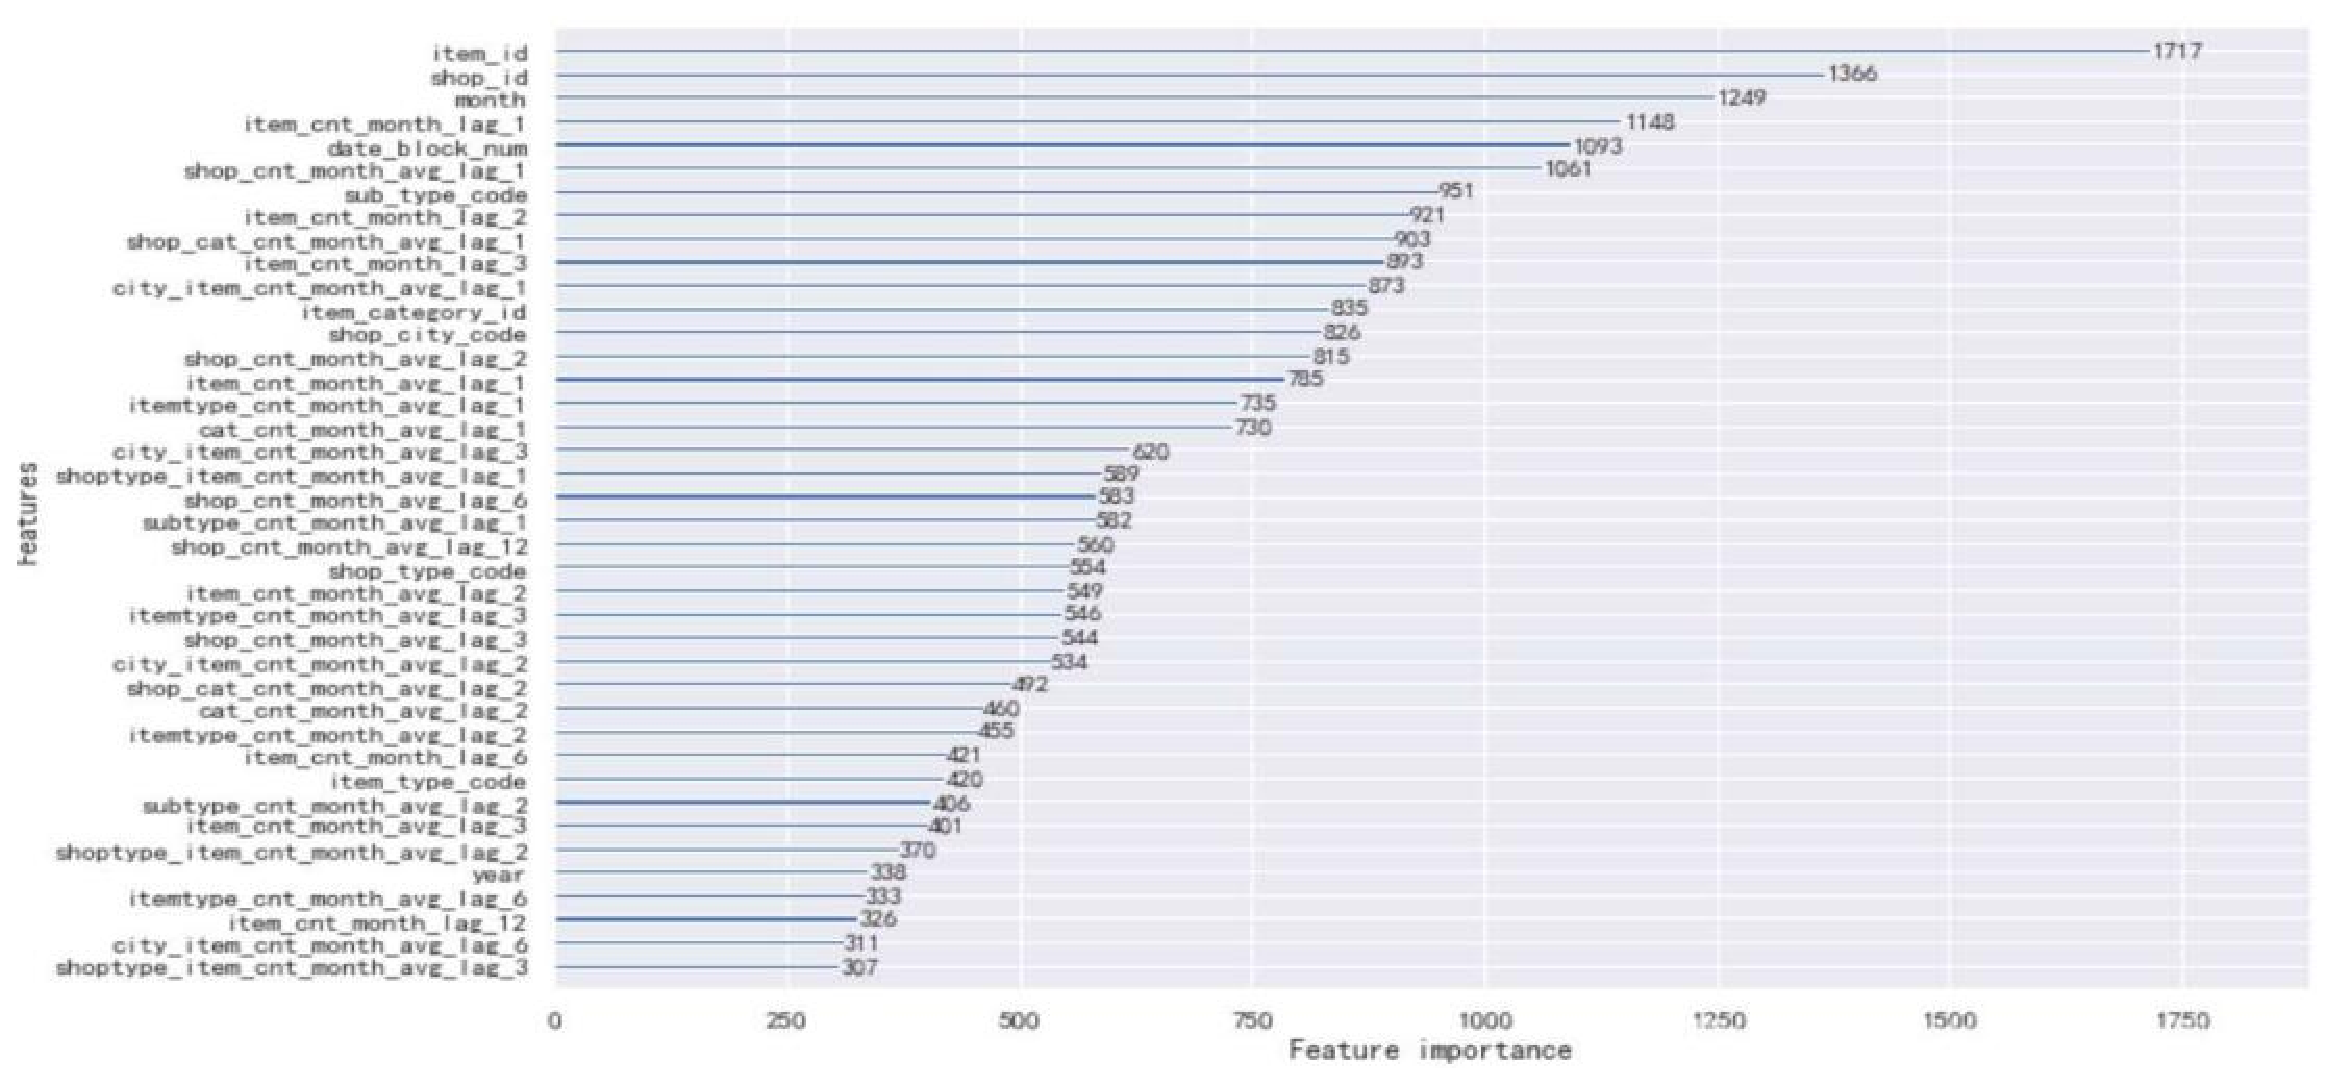
\includegraphics[width=0.9\textwidth,height=0.5\textwidth]{figures/Figure8.eps}\\
    \caption{Feature Importance}
  \end{figure}
  
  %%==========================================================================================
  \begin{note}
  Next,
  I will introduce the non-trivial outlying subspaces.
  Non-Trivial outlying subspaces are multi-dimension subspaces.
  In the subspace,
  the query group's outlying degree is larger than the threshold $\alpha$.
  
  Table $2$ shows that,
  when the threshold $\alpha$ equal four,
  the non-trivial outlying subspace is \{$F_3$, $F_4$\}.
  \end{note}
  %%==========================================================================================
  
  \end{slide}
  %%
  %%==========================================================================================
%%
\begin{slide}{Lightgbm}
  \begin{itemize}
    \item
    train set:date_block_num< 33 \\
    validation set:date_block_num == 33 \\
    test set:date_block_num == 34 \\
    \smallskip
    \item
    score:0.93740
    \smallskip
    \item
    3027/8738
  \end{itemize}
    
    %%==========================================================================================
    \begin{note}
    In order to identify the top-k outlying subspaces,
    we categorize the features into $2$ non-overlapping groups,
    trivial outlying features and non-trivial outlying subspaces.
    
    First, let me introduce the trivial outlying features.
    
    Trivial outlying features are one-dimension subspaces.
    In the subspace,
    the query group's outlying degree is larger than the threshold $\alpha$.
    
    We can see from table $1$,
    when the specified threshold $\alpha = 4$,
    the trivial outlying feature is \{$F_1$\}.
    \end{note}
    %%==========================================================================================
    
    \end{slide}
    %%

%%==========================================================================================
%%
\begin{slide}{Comparison}
  \begin{itemize}
    \item
    1.0485→0.93740
    \smallskip
    \item
    model and feature
    \smallskip
    LightGBM and XGBoost \\
    Add feature:historical feature

  \end{itemize}
    
    %%==========================================================================================
    \begin{note}
    In order to identify the top-k outlying subspaces,
    we categorize the features into $2$ non-overlapping groups,
    trivial outlying features and non-trivial outlying subspaces.
    
    First, let me introduce the trivial outlying features.
    
    Trivial outlying features are one-dimension subspaces.
    In the subspace,
    the query group's outlying degree is larger than the threshold $\alpha$.
    
    We can see from table $1$,
    when the specified threshold $\alpha = 4$,
    the trivial outlying feature is \{$F_1$\}.
    \end{note}
    %%==========================================================================================
    
    \end{slide}
    %%

%%==========================================================================================
% 
% \begin{slide}{Data Feature}
% %Related Work - Outlying Aspects Mining
% \begin{itemize}
% \item
% Existing Methods - \textcolor{orange}{Feature selection}

% \begin{itemize}
% \item
% To distinguish two classes:
% the query point (positive) \& rest of data (negative)
% \end{itemize}
% \vspace{1cm}
% \twocolumn[
% \savevalue{lfrheight}=5cm,
% \savevalue{lfrprop}={
% linestyle=solid,framearc=.2,linewidth=1pt},
% rfrheight=\usevalue{lfrheight},
% rfrprop=\usevalue{lfrprop}
% ]{
% Disadvantages
% \begin{itemize}
% \item
% \smallskip
% Positive and negative classes are \textcolor{orange}{Not} balanced.

% \item
% \smallskip
% \textcolor{orange}{Not} quantify the outlying degree accurately.

% \item
% \smallskip
% \textcolor{orange}{Not} identify group outlying aspects.
% \end{itemize}
% }
% {
% Advantages
% \begin{itemize}
% \item
% \smallskip
% Easy to operate.

% \item
% \smallskip
% Resolve dimensionality bias.
% \end{itemize}
% }
% \end{itemize}

% %%==========================================================================================
% \begin{note}
% Let me introduce two existing methods:
% Feature selection and score-and-search.

% For feature selection,
% the query point can be regarded as positive class and
% the rest of the data can be regarded as negative class,
% selected the features that best distinguish the two classes.

% The advantages of this method are easy to operate,
% and it's able to resolve dimensionality bias.
% However, it has some drawbacks.
% Firstly,
% positive and negative classes are Not balanced,
% secondly,
% it can't quantify the outlying degree correctly.
% Most importantly,
% it doesn't identify group outlying aspects.
% \end{note}
% %%==========================================================================================

% \end{slide}
%%
%%==========================================================================================


%%==========================================================================================
%%
% \begin{slide}[toc=,bm=]{Related Work - Outlying Aspects Mining}

% \begin{itemize}
% \item
% Existing Methods - \textcolor{orange} {Score-and-search}

% \begin{itemize}
% \item
% Define an outlying score function.

% \item
% Search subspaces.
% \end{itemize}
% \bigskip
% \twocolumn[
% \savevalue{lfrheight}=5cm,
% \savevalue{lfrprop}={
% linestyle=solid,framearc=.2,linewidth=1pt},
% rfrheight=\usevalue{lfrheight},
% rfrprop=\usevalue{lfrprop}
% ]{
% Disadvantages
% \begin{itemize}
% \item
% \smallskip
% Dimensionality bias.

% \item
% \smallskip
% Search efficiency is \textcolor{orange}{Not} high (dataset is large).

% \item
% \smallskip
% \textcolor{orange}{Not} identify group outlying aspects.
% \end{itemize}
% }{
% Advantages
% \begin{itemize}
% \item
% \smallskip
% Quantify the outlying degree correctly.

% \item
% \smallskip
% High Comprehensibility.

% \end{itemize}
% }
% \end{itemize}

% %%==========================================================================================
% \begin{note}
% For score-and-search method,
% it defines an outlying score function,
% and then searches for each subspace until it finds out a subspace that
% makes the query point show the best score.

% The advantages of this method are:
% first, it enables to quantify the outlying degree accurately.
% Besides, its comprehensibility is high.

% While the disadvantages include three main aspects:
% the first one is it has dimensionality bias;
% Additionally, its search efficiency is low.
% Last but not least, it doesn't identify group outlying aspects.
% \end{note}
% %%==========================================================================================

% \end{slide}
%%
%%==========================================================================================


%%==========================================================================================
%%
% \begin{slide}[toc=,bm=]{}
% \twocolumn
% {
% Group Outlying Aspects Mining
% \begin{itemize}
% \item
% \smallskip
% Focus on differences between \textcolor{orange}{groups}.

% \item
% \smallskip
% \textcolor{orange}{Multiple} points.
% \medskip
% \end{itemize}
% \vspace{0.75cm}
% %\vspace{0.1cm}
% \begin{figure}
%   \centering
%   \selectcolormodel{rgb}
%   \missingfigure{Testing a long text string.}
%   %\includegraphics[width=0.6\textwidth]{figures//example-basketball-projection.eps}\\
%   \caption{Group Outlying Aspects Target}\label{fig:GroupOutAspect-target}
% \end{figure}
% }
% {
% Outlying Aspects Mining
% \begin{itemize}
% \item
% Concentrates on differences between \textcolor{orange}{objects}.

% \item
% \textcolor{orange}{One} point.
% \end{itemize}
% \bigskip
% \begin{figure}
%   \centering
%   \selectcolormodel{rgb}
%   \missingfigure{Testing a long text string.}
% %  \includegraphics[width=0.5\textwidth]{figures//OutAspect_target.eps}\\
%   \caption{Outlying Aspects Target}\label{fig:OutAspect-target}
% \end{figure}
% }

% %%==========================================================================================
% \begin{note}
% In this research paper,
% we proposed the group outlying aspects mining.
% Now,
% let me summarize the differences between group outlying aspects mining and outlying aspects mining.

% Group outlying aspects mining mainly focuses on the differences between groups.
% But outlying aspects mining mainly concentrates on the differences between objects.
% The target of group outlying aspects mining can be seen as many points.
% While the target of outlying aspects mining can be regarded as one point.

% In the NBA example,
% group outlying aspects mining focuses on the advantages
% or disadvantages of one team,
% however,
% outlying aspects mining focuses on the advantages or disadvantages of one player.
% \end{note}
% %%==========================================================================================

% \end{slide}
%%
%%==========================================================================================


%%==========================================================================================
%%
% \begin{slide}{Challenges (1)}
% %Challenges (1)
% \begin{itemize}
% \item
% How to \textcolor{orange}{represent} the group features.

% \begin{itemize}
% \item
% Can be affected by outlier values.

% \item
% Can \textcolor{orange}{Not} reflect the overall distribution of group features.
% \end{itemize}
% \end{itemize}

% %%==========================================================================================
% \begin{note}
% Based on current existing methods,
% there still remains some research challenges.

% The first one is how to represent the group features
% based on the features of the individuals in the group.

% Although the arithmetic mean of all elements
% in each feature can describe the features of one group.
% It can be affected by outlier values,
% and can't reflect the entire distribution of group features.L
% \end{note}
% %%==========================================================================================

% \end{slide}
%%
%%==========================================================================================


%%==========================================================================================
%%
% \begin{slide}[toc=,bm=]{Challenges (2)}

% \begin{itemize}
% \item
% How to \textcolor{orange}{evaluate} the outlying degree in different aspects.

% \begin{itemize}
% \item
% Need design a scoring function when necessary.

% \item
% Adopting an appropriate scoring function (without dimension bias) remains a problem.

% \end{itemize}
% \end{itemize}

% %%==========================================================================================
% \begin{note}
% The second challenge is how to evaluate the outlying degree of
% the query group between different aspects.

% In that case,
% we need to design a scoring function to measure the outlying degree.
% But adopting an appropriate scoring function without dimension bias still remains a problem.
% \end{note}
% %%==========================================================================================

% \end{slide}
%%
%%==========================================================================================


%%==========================================================================================
%%
% \begin{slide}[toc=,bm=]{Challenges (3)}

% \begin{itemize}
% \item
% How to \textcolor{orange}{improve} the efficiency.

% \begin{itemize}

% \item
% When the dimension of the \textcolor{orange}{data is high},
% the candidate subspace grows exponentially.

% \item
% It will easily go beyond the limits of the computation resources.

% \end{itemize}
% \end{itemize}

% %%==========================================================================================
% \begin{note}
% The third challenge is how to improve efficiency.

% To be specific,
% when the dimension of data is high,
% the candidate subspace increase dramatically,
% so that it is very easy to exceed the limit of computer resources.
% \end{note}
% %%==========================================================================================

% \end{slide}
%%
%%==========================================================================================


% \section{GOAM Algorithm}


% %%==========================================================================================
% %%
% \begin{slide}[toc=,bm=]{}

% Framework of GOAM algorithm:

% \bigskip

% \begin{figure}
%   \centering
%   \selectcolormodel{rgb}
%   \missingfigure{Testing a long text string.}
% %  \includegraphics[width=0.55\textwidth]{figures//framework1.eps}\\
%   \caption{Framework of GOAM Algorithm} \label{framework}
% \end{figure}

% %%==========================================================================================
% \begin{note}
% In order to tackle the above issues,
% GOAM algorithm is involved.

% Let's have a look at the framework of this algorithm.
% The first step is to use the histogram to represent the group features
% based on all individuals in the group.

% Following that,
% we utilize the earth mover distances to measure the
% outlying degree between groups.
% This is the second step:
% outlying degree scoring.

% The last step is to identify the outlying aspects.

% \end{note}
% %%==========================================================================================

% \end{slide}
%%
%%==========================================================================================


%%==========================================================================================
%%
% \begin{slide}{Step One - Group Feature Extraction}
% %Step One - Group Feature Extraction}
% \begin{itemize}
% \item
% \smallskip
% Suppose $f_1$, $f_2$, $f_3$ are three features of $G_q$.

% $f_1$: \{$x_1, x_2, x_3, x_4, x_5, x_2, x_3, x_4, x_1, x_2$\} \\

% $f_2$: \{$y_2, y_2, y_1, y_2, y_3, y_3, y_5, y_4, y_4, y_2$\} \\

% $f_3$: \{$z_1, z_4, z_2, z_4, z_5, z_3, z_1, z_2, z_4, z_2$\} \\
% \end{itemize}

% \begin{figure}[htbp]
%     \centering
%     \subfigure[$f_1$]{
%         \selectcolormodel{rgb}
%         \missingfigure[figwidth=5.5cm]{Test.}
%         %\includegraphics[width=0.25\textwidth]{figures//frequency-distribution-feature1.eps}
%         \label{fig:fre-dis-f1}
%     }
%     \subfigure[$f_2$]{
%         \selectcolormodel{rgb}
%         \missingfigure[figwidth=5.5cm]{Test.}
%         \label{fig:fre-dis-f2}
%     }
%     \subfigure[$f_3$]{
%         \selectcolormodel{rgb}
%         \missingfigure[figwidth=5.5cm]{Test.}
%         \label{fig:fre-dis-f3}
%     }
%     \caption{Histogram of $G_q$ on three features}
%     \label{fig:fre-dis-each-feature}
% \end{figure}

% %%==========================================================================================
% \begin{note}
% Now, let me specifically explain what each step means.
% The first step is group feature extraction.
% we can take one group extraction as an example.

% We suppose to use $f_1$, $f_2$, $f_3$ to represent three features of $G_q$.
% The values of $f_1$ are {$x_1$, $x_2$, $x_3$, $x_4$} and so on.
% And the values of $f_2$ are {$y_2$, $y_2$, $y_1$, $x_2$} and so on.

% For feature $f_1$,
% we use the histogram to illustrate feature $f_1$ after
% counting the frequency of each value,
% as show in figure 6 (a).

% Similarly,
% we can also extract other features of the group
% according to feature $f_1$.
% \end{note}
% %%==========================================================================================

% \end{slide}
%%
%%==========================================================================================


%%==========================================================================================
%%
% \begin{slide}{Step Two - Outlying Degree Scoring}
% %Step Two - Outlying Degree Scoring
% \begin{itemize}
% \item
% Calculate Earth Mover Distance

% \begin{itemize}
% \item
% Represent one feature among different groups

% \item
% Purpose: calculate the minimum mean distance
% \end{itemize}

% \begin{figure}
%    \selectcolormodel{rgb}
%    \missingfigure{Make a sketch of the structure of a trebuchet.}
% %  \includegraphics[width=0.4\textwidth]{figures//example3.eps}\\
%    \caption{EMD of one feature}\label{EMD}
% \end{figure}
% \end{itemize}

% %%==========================================================================================
% \begin{note}
% The second step is outlying degree scoring,
% which is to evaluate the outlying degree between the target group and competitive groups.

% First,
% we calculate the earth mover distance of one feature in different groups.

% The earth mover distance reflects the minimum mean distance between
% the target group and other groups on one feature.

% Later on,
% we utilize the EMD to measure the differences between groups.
% \end{note}
% %%==========================================================================================

% \end{slide}
%%
%%==========================================================================================


%%==========================================================================================
%%
% \begin{slide}[toc=,bm=]{Step Two - Outlying Degree Scoring}

% \begin{itemize}
% \item
% Calculate the outlying degree

% \vspace{1.2cm}

% \begin{centering}

% $ OD(G_q) = \sum_{1}^{n}EDM(h_{q_s}, h_{k_s}) $

% \end{centering}

% \begin{itemize}
% \item
% n $\Leftrightarrow$ the number of contrast groups.

% \item
% $h_{k_s}$  $\Leftrightarrow$ the histogram representation of $G_k$ in the subspace s.

% \end{itemize}
% \end{itemize}

% %%==========================================================================================
% \begin{note}
% Base on the earth mover distance,
% we can calculate the outlying degree using the formula shown on the screen.

% This formula is the outlying degree scoring function,
% n represents the number of competitive groups.
% $h_{k_s}$ is the histogram of $G_k$ in the subspace s.
% \end{note}
% %%==========================================================================================

% \end{slide}
%%
%%==========================================================================================


%%==========================================================================================
%%
% \begin{slide}{Step Three - Outlying Aspects Identification}
% %Step Three - Outlying Aspects Identification
% \begin{itemize}
% \item
% Identify group outlying aspects mining based on the value
% of outlying degree.

% \item
% The greater the outlying degree is,
% the more likely it is group outlying aspect.
% \end{itemize}

% %%==========================================================================================
% \begin{note}
% Next,
% let me talk about the third step.

% In this step,
% we identify the group outlying aspects according to the value of the outlying degree.

% If a feature's outlying degree is greater,
% it is more likely to be a group outlying aspect.
% \end{note}
% %%==========================================================================================

% \end{slide}
%%
%%==========================================================================================


%%==========================================================================================
%%
% \begin{slide}[toc=,bm=]{Pseudo code}

% \begin{itemize}
% \item
% Pseudo code of GOAM algorithm

% \end{itemize}

% \begin{figure}
%   \centering
%   \selectcolormodel{rgb}
%   \missingfigure[figwidth=16cm]{Testing a long text string}
%   %\includegraphics[width=0.75\textwidth]{figures//GOAM.eps}\\
%   %\caption{GOAM Algorithm}\label{OS-Identification}
% \end{figure}

% %%==========================================================================================
% \begin{note}
% Last,
% we use the outlying degree to identify the specific group outlying aspects.

% The pseudo code of GOAM algorithm is as follows.
% The input is the group data,
% the output is outlying aspects of specific group ($G_1$).

% The details of the algorithm I will use an example to explain.
% \end{note}

% %%==========================================================================================
% \end{slide}
%%
%%==========================================================================================


%%==========================================================================================
%%
% \begin{slide}[toc=,bm=]{Illustration}
% % Outlying Aspects Identification
% \begin{table}
% \setlength{\abovecaptionskip}{0pt}
% \setlength{\belowcaptionskip}{10pt}
% \centering
% \caption{Original Dataset}
% \begin{tabular}{ccccc | ccccc}
%   \toprule
%   $G_1$ & $F_1$ & $F_2$ & $F_3$ & $F_4$ & $G_2$ & $F_1$ & $F_2$ & $F_3$ & $F_4$ \\
%   \midrule
%    &10 & 8 & 9 & 8 & &7 & 7 & 6 & 6 \\
%    &9  & 9 & 7 & 9 & &8 & 9 & 9 & 8 \\
%    &8  & 10& 8 & 8 & &6 & 7 & 8 & 9  \\
%    &8  & 8 & 6 & 7 & &7 & 7 & 7 & 8  \\
%    &9  & 9 & 9 & 8 & &8 & 6 & 6 & 7  \\
%    \midrule
%    $G_3$ & $F_1$ & $F_2$ & $F_3$ & $F_4$ & $G_4$ & $F_1$ & $F_2$ & $F_3$ & $F_4$ \\
%    \midrule
%    &8 & 10 & 8 & 8 & &9 & 8 & 8 & 8\\
%    &9 & 9  & 7 & 9 & &7 & 7 & 7 & 9\\
%    &10& 9  & 10& 7 & &8 & 6 & 6 & 8\\
%    &9 & 10 & 8 & 6 & &9 & 8 & 8 & 7\\
%    &9 & 9  & 7 & 9 & &8 & 7 & 9 & 8\\
%   \bottomrule
% \end{tabular}
% \end{table}

% %%==========================================================================================
% \begin{note}
% Next,
% let me use an example to explain GOAM algorithm.

% Suppose we have four groups.
% Each group has four features,
% and
% the specific values are shown in table $3$.
% \end{note}
% %%==========================================================================================

% \end{slide}
%%
%%==========================================================================================


%%==========================================================================================
%%
% \begin{slide}[toc=,bm=]{Illustration}

% \setlength{\abovecaptionskip}{0pt}
% \setlength{\belowcaptionskip}{10pt}
% \centering
% \begin{table}
% \caption{outlying degree of each possible subspaces}

% \begin{tabular}{c|c|c|c}
%   \toprule
%   % after \\: \hline or \cline{col1-col2} \cline{col3-col4}
%   Feature & Outlying Degree & Feature & Outlying Degree \\
%   \midrule
%   \textcolor{orange}{\{$F_1$\}}  & 4.351  & \{$F_2, F_3$\}  & 4.023 \\
%   \{$F_2$\}  & 2.012                      & \textcolor{orange}{\{$F_3, F_4$\}} & 4.324 \\
%   \{$F_3$\}  & 1.392                      & \{$F_2, F_4$\} & 2.018 \\
%   \{$F_4$\}  & 2.207                      & \{$F_2, F_3, F_4$\} & 2.012 \\
%   \bottomrule
% \end{tabular}
% \end{table}

% \bigskip

% \twocolumn{
% \begin{itemize}
% \item
% Search process:\\
% $OD(\{$$F_1$$\}) > \alpha$, save to $T_1$.\\
% $OD(\{$$F_2$$\}) < \alpha$, save to $C_1$.\\
% $OD(\{$$F_3$$\}) < \alpha$, save to $C_2$. \\
% $OD(\{$$F_4$$\}) < \alpha$, save to $C_3$. \\
% \end{itemize}}
% {
% \vspace{.75cm}
% $OD(\{$$F_2, F_3$$\}) > \alpha$, save to $N_1$. \\
% $OD(\{$$F_3, F_4$$\}) > \alpha$, save to $N_2$. \\
% $OD(\{$$F_2, F_4$$\}) < \alpha$, remove. \\
% $OD(\{$$F_2, F_3, F_4$$\}) < \alpha$, remove. \\
% }
% %Sort $N_i$ in descending order,
% %add subspace with top-k outlying degree in $N_i$ to $O_k$

% %%==========================================================================================
% \begin{note}
% According to the outlying degree scoring function,
% we can get the outlying degree of each possible subspace.

% So that we can filter out the candidate subspaces.
% Next is to sort the candidate subspaces in
% descending order and then we pick out the top-k subspaces.

% The result is as shown in table $4$.
% As a result,
% the top-1 group outlying aspect is \{$F_1$\}.
% The top-2 group outlying aspects include
% trivial feature \{$F_1$\},
% and non-trivial subspace \{$F_3, F_4$\}.
% \end{note}
% %%==========================================================================================

% \end{slide}
%%
%%==========================================================================================


%%==========================================================================================
%%
% \begin{slide}[toc=,bm=]{Strengths of GOAM Algorithm}
% \begin{itemize}
% \item
% \textcolor{orange}{Reduction of Complexity}

% \begin{itemize}
% \item
% Bottom-up search strategy.

% \item
% Reduce the size of candidate subspaces.

% \end{itemize}

% \item
% \textcolor{orange}{Efficiency}

% \begin{itemize}
% \item
% Before: $O(2^d)$  \\
% Now:    $O(d*n^{2})$

% \end{itemize}
% \end{itemize}

% %%==========================================================================================
% \begin{note}
% In terms of the strengths of GOAM algorithm.

% I would like to talk about two main advantages of this algorithm.
% First is the reduction of complexity.
% GOAM algorithm utilizes the bottom up search method;
% what's more,
% it can reduce the size of candidate subspaces.

% Second is efficiency.
% The previous time complexity is O($2^d$);
% however,
% current time complexity if only O($d*n^2$).
% \end{note}
% %%==========================================================================================

% \end{slide}
%%
%%==========================================================================================


% \section{Evaluation Results}


% %%==========================================================================================
% %%
% \begin{slide}[toc=,bm=]{Evaluation}

% \begin{center}
% \begin{itemize}

% \item
% \smallskip
% \large
% {$Accuracy = \frac{P}{T}$ \\
% P: Identified outlying aspects \\

% T: Real outlying aspects}

% \end{itemize}
% \end{center}

% %%==========================================================================================
% \begin{note}
% Before showing the experiment results,
% I will introduce the evaluation of the experiment.

% We use accuracy formula to make comparisons between GOAM algorithm
% and outlying aspect mining method.
% In the accuracy formula,
% P stands for identified outlying aspects;
% and T means the real outlying aspects.
% \end{note}
% %%==========================================================================================

% \end{slide}
%%
%%==========================================================================================


%%==========================================================================================
%%
% \begin{slide}{Synthetic Dataset}

% \begin{itemize}
% \item Synthetic Dataset and Ground Truth
% \end{itemize}

% \begin{table}
% \setlength{\abovecaptionskip}{0pt}
% \setlength{\belowcaptionskip}{10pt}
% \centering
% \caption{Synthetic Dataset and Ground Truth}

% \begin{tabular}{p{2.8cm}p{0.9cm}p{0.9cm}p{0.9cm}p{0.9cm}p{0.9cm}p{0.9cm}p{0.9cm}p{0.9cm}}
% \hline
%   % after \\: \hline or \cline{col1-col2} \cline{col3-col4} ...
%   Query group  & $\mathbf{F_1}$ & $\mathbf{F_2}$ & $F_3$ & $\mathbf{F_4}$ & $F_5$ & $F_6$ & $F_7$ & $F_8$\\
% \hline
%   $i_1$   & \bf{10} & \bf{8}  & 9  & \bf{7}  & 7 & 6 & 6  & 8\\
%   $i_2$   & \bf{9}  & \bf{9}  & 7  & \bf{8}  & 9 & 9 & 8  & 9\\
%   $i_3$   & \bf{8}  & \bf{10} & 8  & \bf{9}  & 6 & 8 & 7  & 8\\
%   $i_4$   & \bf{8}  & \bf{8}  & 6  & \bf{7}  & 8 & 8 & 6  & 7\\
%   $i_5$   & \bf{9}  & \bf{9}  & 9  & \bf{7}  & 7 & 7 & 8  & 8\\
%   $i_6$   & \bf{8}  & \bf{10} & 8  & \bf{8}  & 6 & 6 & 8  & 7\\
%   $i_7$   & \bf{9}  & \bf{9}  & 7  & \bf{9}  & 8 & 8 & 8  & 7\\
%   $i_8$   & \bf{10} & \bf{9}  & 10 & \bf{7}  & 7 & 7 & 7  & 7\\
%   $i_9$   & \bf{9}  & \bf{10} & 8  & \bf{8}  & 7 & 6 & 7  & 7\\
%   $i_{10}$& \bf{9}  & \bf{9}  & 7  & \bf{7}  & 7 & 8 & 8  & 8\\
% \hline
% \end{tabular}
% \end{table}

% %%==========================================================================================
% \begin{note}
% Now,
% I am gonna use a synthetic dataset to verify our method.

% The dataset we used in our experiment contains $10$ groups,
% each group consists of $10$ members,
% and each member has $8$ features: $F_1$ to $F_8$.

% Table $5$ shows the original data of one group,
% and the bold features represent the ground truth,
% The ground truth include trivial outlying feature \{$F_1$\},
% and non-trivial outlying subspace \{$F_2$, $F_4$\}.
% \end{note}
% %%==========================================================================================

% \end{slide}
%%
%%==========================================================================================


%%==========================================================================================
%%
% \begin{slide}[toc=,bm=]{Synthetic Dataset Results}

% \begin{table}[tb]
% \setlength{\abovecaptionskip}{0pt}
% \setlength{\belowcaptionskip}{10pt}
% \centering
% \caption{The experiment result on synthetic dataset}

% \begin{tabular}{ c | c | c | c }
% \toprule
%   % after \\: \hline or \cline{col1-col2} \cline{col3-col4} ...
%   Method     &  Truth Outlying Aspects    & Identified Aspects & Accuracy      \\
% \midrule
%   GOAM       &  $\{F_1\}$, $\{F_2F_4\}$   &  $\{F_1\}$, $\{F_2F_4\}$    & 100\%    \\

% Arithmetic Mean based OAM &  $\{F_1\}$, $\{F_2F_4\}$   &  $\{F_4\}$, $\{F_2\}$    &  0\% \\

% Median based OAM &  $\{F_1\}$, $\{F_2F_4\}$   &  $\{F_2\}$, $\{F_4\}$    &           0\% \\
% \bottomrule
% \end{tabular}
% \end{table}

% %%==========================================================================================
% \begin{note}
% From table $6$,
% we can see that GOAM method can identify the trivial outlying features
% and non-trivial outlying subspaces accurately and
% it is obvious from the table that the accuracy of GOAM is the best,
% which is 100\%.

% This is because the outlying aspects mining method
% can't obtain the features of a group and the scoring function
% is based on point to point metric.
% Therefore,
% it is not suitable for group outlying aspects mining.
% \end{note}
% %%==========================================================================================

% \end{slide}
%%
%%==========================================================================================


%%==========================================================================================
%%
% \begin{slide}{NBA Dataset}
% Data Collection
% \begin{description}[type=1]
% \item
% Source\\
% \qquad
% \emph{Yahoo Sports} website (\url{http://sports.yahoo.com.cn/nba})

% \item
% Data

% \begin{itemize}
%  \item Extract NBA teams' data until March 30, 2018;
%  \item 6 divisions;
%  \item 12 features (eg: \emph{Point Scored}).
% \end{itemize}
% \end{description}

% %%==========================================================================================
% \begin{note}
% Next,
% I will illustrate it further by applying the GOAM algorithm to the NBA dataset.
% The data was collected from Yahoo Sports website.

% In our experiment,
% a web crawler was deployed to extract data
% for all NBA teams until March 30, 2018.
% The data includes all teams from the six divisions,
% and each player in the team has 12 features,
% such as point scored, field goal\dots
% \end{note}
% %%==========================================================================================

% \end{slide}
%%
%%==========================================================================================


%%==========================================================================================
%%
% \begin{slide}[toc=,bm=]{NBA Dataset}
% The detail features are as follows:

% \begin{table}[tb]
% \setlength{\abovecaptionskip}{0pt}
% \setlength{\belowcaptionskip}{10pt}
% \centering
% \caption{Collected data of Brooklyn Nets Team}

% \begin{tabular}{p{0.9cm}p{0.9cm}p{0.9cm}p{0.9cm}p{0.9cm}p{0.9cm}p{0.9cm}p{0.9cm}p{0.9cm}p{0.9cm}p{0.9cm}p{0.9cm}}
% \hline
%   Pts & FGA & FG\% & 3FA & 3PT\% & FTA & FT\% & Reb & Ass & To & Stl & Blk \\
% \hline
%   18   & 12    & 42 &2.00 & 50 & 7.00 & 100& 0& 4& 3& 0& 0 \\
%   15.7 & 14.07 & 41 &5.45 & 32 & 3.05 & 75 & 3.98& 5.1& 2.98& 0.69& 0.36\\
%   14.5 & 11.1  & 47 &0.82 & 26 & 4.87 & 78 & 6.82& 2.4& 1.74& 0.92& 0.66 \\
%   13.5 & 10.8  & 42 &5.37 & 37 & 3.38 & 77 & 6.66& 2& 1.38& 0.83& 0.42 \\
%   12.7 & 10.59 & 39 &5.36 & 33 & 3.37 & 82 & 3.24& 6.6& 1.56& 0.89& 0.31 \\
%   12.6 & 10.93 & 40 &6.94 & 37 & 1.70 & 84 & 4.27& 1.5& 1.06& 0.61& 0.44 \\
%   12.2 & 10.39 & 44 &3.42 & 35 & 2.70 & 72 & 3.79& 4.1& 2.15& 1.12& 0.32 \\
%   10.6 & 7.85  & 49 &4.51 & 41 & 1.35 & 83 & 3.34& 1.6& 1.15 & 0.45& 0.24 \\
% \hline
% \end{tabular}
% \end{table}

% %%==========================================================================================
% \begin{note}
% Table $7$ shows part of the collected data.
% From this table,
% we can see that the feature values are continuous.
% \end{note}
% %%==========================================================================================

% \end{slide}
%%
%%==========================================================================================


%%==========================================================================================
%%
% \begin{slide}[toc=,bm=]{NBA Dataset}
% \begin{itemize}
% \item Data Preprocess
% \end{itemize}

% \begin{table}
% \setlength{\abovecaptionskip}{0pt}
% \setlength{\belowcaptionskip}{10pt}
% \centering
% \caption{The bins that used to discrete data of each feature}

% \begin{tabular}{p{2.5cm}p{2cm}p{1.8cm}p{2cm}p{1.8cm}p{1.8cm}p{1.8cm}}
% \hline
%   Labels & Pts & FGA & FG\% & 3FA & 3PT\% & FTA  \\
% \hline
%   low &  [0,5]& [0,4] & [0,0.35] & [0,1.0] & [0,0.2] & [0,1.0] \\
%   medium& (5,10]& (4,7] & (0.35,0.45] & (1.0,2.5]& (0.2,0.3] & (1.0,1.5] \\
%   high &  (10,15] & (7,10] & (0.45,0.5] & (2.5,3.5]& (0.3,0.35]& (1.5,2.5] \\
%   very high&(15,$+\infty$]& (10,$+\infty$] & (0.5,1] & (3.5,$+\infty$] & (0.35,1] & (2.5,$+\infty$] \\
% \hline
%  Labels & FT\% & Reb & Ass & To & Stl & Blk \\
% \hline
%   low   & [0,0.6] & [0,2.0] & [0,1.0] & [0,0.6] & [0,0.2] & [0,0.25] \\
%   medium& (0.6,0.65]& (2,5] & (1,2] & (0.6,0.9] & (0.2,0.5] & (0.25,0.5] \\
%   high  & (0.65,0.75] & (5,6] & (2,4] & (0.9,1.7] & (0.6,0.75] & (0.5,0.7] \\
%   very high& (0.75,1] & (6,$+\infty$] & (4,$+\infty$] & (1.7,$+\infty$] & (0.75,$+\infty$] & (0.7,$+\infty$]\\
% \hline
% \end{tabular}
% \end{table}

% %%==========================================================================================
% \begin{note}
% For those features with continuous values,
% we use the binning method to discretize them,
% the results are shown in table $8$.

% Once the data was prepared,
% we added three teams in the eastern division
% and three teams in the western division into the query group,
% the other teams together belonged to the contrast groups.
% \end{note}
% %%==========================================================================================

% \end{slide}
%%
%%==========================================================================================


%%==========================================================================================
%%
% \begin{slide}[toc=,bm=]{NBA Dataset Results}

% \begin{table}[htbp]
% \setlength{\abovecaptionskip}{0pt}
% \setlength{\belowcaptionskip}{10pt}
% \centering
% \caption{The identified outlying aspects of groups}

% \begin{tabular}{ccc}
% \hline
%   Teams                   & Trivial Outlying Aspects  & NonTrivial Outlying Aspects    \\
% \hline
%   Cleveland Cavaliers     & \{3FA\}                   & \{FGA, FT\%\}, \{FGA, FG\%\} \\
%   Orlando Magic           & \{Stl\}                   & None                         \\
%   Milwaukee Bucks         & \{To\}, \{FTA\}           & \{FGA, FTA\}, \{3FA, FTA\}     \\
%   Golden State Warriors   & \{FG\%\}                  & \{FT\%, Blk\}, \{FGA, 3PT\%, FTA\}\\
%   Utah Jazz               & \{Blk\}                   & \{3FA, 3PT\%\}                    \\
%   New Orleans Pelicans    & \{FT\%\}, \{FTA\}         & \{FTA, Stl\}, \{FTA, To\}          \\
% \hline
% \end{tabular}
% \end{table}

% %%==========================================================================================
% \begin{note}
% We can see the identified group outlying aspects of each team from table $9$.
% It is very clear that the GOAM algorithm can identify the
% Trivial Outlying Aspects and Non-Trivial Outlying Aspects of each team.
% \end{note}
% %%==========================================================================================

% \end{slide}
%%
%%==========================================================================================


% \section{Conclusion}

% %%==========================================================================================
% %%
% \begin{slide}[toc=,bm=]{Conclusion}
% \begin{itemize}
% \item
% \smallskip
% Formalize the problem of \emph{Group Outlying Aspects Mining} by
% extending outlying aspects mining;

% \item
% \smallskip
% Propose a novel method \textcolor{orange}{GOAM algorithm} to solve the
% \emph{Group Outlying Aspects Mining} problem;

% \item
% \smallskip
% Utilize the pruning strategies to reduce time complexity.

% \end{itemize}

% %%==========================================================================================
% \begin{note}
% In conclusion,
% we firstly formalized the problem of
% group outlying aspects mining,

% Then proposed a novel method GOAM algorithm to address the problem of
% group outlying aspects mining,
% and the proposed method use pruning to reduce time complexity
% while identifying the suitable set of outlying features for the interested group.

% Thank you and any question?
% \end{note}
% %%==========================================================================================

% \end{slide}
%%
%%==========================================================================================


%%==========================================================================================
%
% \begin{slide}[toc=,bm=]{Questions?}
% \begin{center}
% \begin{figure}
%     \animategraphics[autoplay, loop, height=0.4\textheight]{5}{./graphics//gif//question//q_}{1}{30}
% \end{figure}
% \end{center}
% \end{slide}
%%
%%==========================================================================================


%%==========================================================================================
% TODO: Contact Page
% \begin{wideslide}[toc=,bm=]{Contact Information}
% \centering
% \vspace{\stretch{1}}
% \twocolumn[
% lcolwidth=0.35\linewidth,
% rcolwidth=0.65\linewidth
% ]
% {
% % \centerline{
\includegraphics[scale=.2]{tulip-logo.eps}}
% }
% {
% \vspace{\stretch{1}}
% Associate Professor Gang Li\\
% School of Information Technology\\
% Deakin University, Australia
% \begin{description}
%  \item[\textcolor{orange}{\faEnvelope}] \href{mailto:gangli@tulip.org.au}
%  {\textsc{\footnotesize{gangli@tulip.org.au}}}

%  \item[\textcolor{orange}{\faHome}] \href{http://www.tulip.org.au}
%  {\textsc{\footnotesize{Team for Universal Learning and Intelligent Processing}}}
% \end{description}
% }
% \vspace{\stretch{1}}
% \end{wideslide}

\end{document}

\endinput
